\PassOptionsToPackage{enable-debug,check-declarations}{expl3}
\RequirePackage{pdfmanagement-testphase}
\DeclareDocumentMetadata {  }
\ExplSyntaxOn
\pdfmanagement_add:nnn{Catalog}{Lang}{(enUS)}
\ExplSyntaxOff

% xmp metadata for pdf
% Originally used \usepackage[a-2a]{pdfx}
% \usepackage{hyperxmp} replaced it
% \RequirePackage{pdfmanagement-testphase} replaced it

\documentclass[11pt,
  english,
  a4paper,
]{article}
\usepackage{sa4all}
\usepackage{amsmath,amssymb,array}
\usepackage{booktabs}

% From tagged-template.latex
\usepackage{lmodern}
\usepackage{ifxetex,ifluatex}
\ifnum 0\ifxetex 1\fi\ifluatex 1\fi=0 % if pdftex
  \usepackage[T1]{fontenc}
  \usepackage[utf8]{inputenc}
  \usepackage{textcomp} % provide euro and other symbols
\else % if luatex or xetex
  \usepackage{unicode-math}
  \defaultfontfeatures{Scale=MatchLowercase}
  \defaultfontfeatures[\rmfamily]{Ligatures=TeX,Scale=1}
\fi

% Use upquote if available, for straight quotes in verbatim environments
\IfFileExists{upquote.sty}{\usepackage{upquote}}{}
\IfFileExists{microtype.sty}{% use microtype if available
  \usepackage[]{microtype}
  \UseMicrotypeSet[protrusion]{basicmath} % disable protrusion for tt fonts
}{}
\makeatletter
\@ifundefined{KOMAClassName}{% if non-KOMA class
  \IfFileExists{parskip.sty}{%
    \usepackage{parskip}
  }{% else
    \setlength{\parindent}{0pt}
    \setlength{\parskip}{6pt plus 2pt minus 1pt}}
}{% if KOMA class
  \KOMAoptions{parskip=half}}
\makeatother
\usepackage{xcolor}
\IfFileExists{xurl.sty}{\usepackage{xurl}}{} % add URL line breaks if available
\hypersetup{
  pdftitle={Status of Arrowtooth flounder (Atheresthes stomias) in the Gulf of Alaska for 2021},
  pdflang={en},
  hidelinks,
  pdfcreator={LaTeX via pandoc}}
\urlstyle{same} % disable monospaced font for URLs
\usepackage{longtable}
% Correct order of tables after \paragraph or \subparagraph
\usepackage{etoolbox}
\makeatletter
\patchcmd\longtable{\par}{\if@noskipsec\mbox{}\fi\par}{}{}
\makeatother
% Allow footnotes in longtable head/foot
\IfFileExists{footnotehyper.sty}{\usepackage{footnotehyper}}{\usepackage{footnote}}
\makesavenoteenv{longtable}
\usepackage{graphicx}
\makeatletter
\def\maxwidth{\ifdim\Gin@nat@width>\linewidth\linewidth\else\Gin@nat@width\fi}
\def\maxheight{\ifdim\Gin@nat@height>\textheight\textheight\else\Gin@nat@height\fi}
\makeatother
% Scale images if necessary, so that they will not overflow the page
% margins by default, and it is still possible to overwrite the defaults
% using explicit options in \includegraphics[width, height, ...]{}
\setkeys{Gin}{width=\maxwidth,height=\maxheight,keepaspectratio}
% Set default figure placement to htbp
\makeatletter
\def\fps@figure{htbp}
\makeatother
\setlength{\emergencystretch}{3em} % prevent overfull lines
\providecommand{\tightlist}{%
  \setlength{\itemsep}{0pt}\setlength{\parskip}{0pt}}
\setcounter{secnumdepth}{5}
\ifxetex
  % Load polyglossia as late as possible: uses bidi with RTL langages (e.g. Hebrew, Arabic)
  \usepackage{polyglossia}
  \setmainlanguage[]{english}
\else
  \usepackage[shorthands=off,main=english]{babel}
\fi

%Define cslreferences environment, required by pandoc 2.8
%https://github.com/rstudio/rmarkdown/issues/1649
\newlength{\csllabelwidth}
\setlength{\csllabelwidth}{3em}
\newlength{\cslhangindent}
\setlength{\cslhangindent}{1.5em}
% for Pandoc 2.8 to 2.10.1
\newenvironment{cslreferences}%
  {}%
  {\par}
% For Pandoc 2.11+
\newenvironment{CSLReferences}[2] % #1 hanging-ident, #2 entry spacing
 {% don't indent paragraphs
  \setlength{\parindent}{0pt}
  % turn on hanging indent if param 1 is 1
  \ifodd #1 \everypar{\setlength{\hangindent}{\cslhangindent}}\ignorespaces\fi
  % set entry spacing
  \ifnum #2 > 0
  \setlength{\parskip}{#2\baselineskip}
  \fi
 }%
 {}
\usepackage{calc}  % for \widthof, \maxof in minipage
\newcommand{\CSLBlock}[1]{#1\hfill\break}
\newcommand{\CSLLeftMargin}[1]{\parbox[t]{\csllabelwidth}{#1}}
\newcommand{\CSLRightInline}[1]{\parbox[t]{\linewidth - \csllabelwidth}{#1}\break}
\newcommand{\CSLIndent}[1]{\hspace{\cslhangindent}#1}


\providecommand{\tightlist}{%
  \setlength{\itemsep}{0pt}\setlength{\parskip}{0pt}}


\date{}
\newcommand{\trTitle}{Status of Arrowtooth flounder (\emph{Atheresthes stomias}) in the Gulf of Alaska for 2021}
\newcommand{\trYear}{2021}
\newcommand{\trMonth}{May}
\newcommand{\trAuthsLong}{true}
\newcommand{\trAuthsBack}{Shotwell, K}
\newcommand{\trCitation}{
\begin{hangparas}{1em}{1}
\trAuthsBack{}. \trYear{}. \trTitle{}. Pacific Fisheries Management Council, Portland, Oregon. \pageref{LastPage}{}\,p.
\end{hangparas}}

\AtBeginDocument{\tagstructbegin{tag=Document}}
\AtEndDocument{\tagstructend}
\pretocmd{\maketitle}{\tagstructbegin{tag=H1}\tagmcbegin{tag=H1}}{}{}
\apptocmd{\maketitle}{\tagmcend\tagstructend}{}{}

\begin{document}

%%%%% Frontmatter %%%%%

% Footnote symbols in front matter
\renewcommand*{\thefootnote}{\fnsymbol{footnote}}

\small
\thispagestyle{empty}
\pagenumbering{roman}
\noindent
\begin{center}
\title{Status of Arrowtooth flounder (\emph{Atheresthes stomias}) in the Gulf of Alaska for 2021}
% \textnormal{\MakeTextUppercase{\trTitle{}}}
\vspace{1.5cm}
{\Large\textbf\newline{Status of Arrowtooth flounder (\emph{Atheresthes stomias}) in the Gulf of Alaska for 2021}}
\vfill
by\\
Kalei Shotwell\textsuperscript{1}\vfill
\textsuperscript{1}.na.character\vfill
\trMonth{} \trYear{}
\end{center}
\clearpage

% Fourth page: Colophon
\thispagestyle{empty}
\vspace*{\fill}
\begin{center}
\copyright{} Pacific Fisheries Management Council, \trYear{}\\
\end{center}
\par
\bigskip
\noindent
Correct citation for this publication:
\bigskip
\par
\trCitation{}
\clearpage

% Add TOC to pdf bookmarks (clickable pdf)
\pdfbookmark[1]{\contentsname}{toc}

% Table of contents page, lists of figures and tables
\tableofcontents\clearpage
\listoffigures \listoftables \clearpage
\label{TRlastRoman}
\clearpage

% Table of contents
\newpage
\thispagestyle{empty} % to remove page number

% Settings for the main document
\pagenumbering{arabic}  % Regular page numbers
\pagestyle{plain}  % No page number on first page of main document, use 'empty'
\renewcommand*{\thefootnote}{\arabic{footnote}}  % Back to numeric footnotes
\setcounter{footnote}{0}  % And start at 1
\renewcommand{\headrulewidth}{0.5pt}
\renewcommand{\footrulewidth}{0.5pt}
%\pagestyle{fancy}\fancyhead[c]{Draft: Do not cite or circulate}

\newcommand{\lt}{\ensuremath <}
\newcommand{\gt}{\ensuremath >}

\tagstructbegin{tag=H1}\tagmcbegin{tag=H1}

\hypertarget{executive-summary}{%
\section*{Executive Summary}\label{executive-summary}}
\addcontentsline{toc}{section}{Executive Summary}

\leavevmode\tagmcend\tagstructend

\tagstructbegin{tag=H2}\tagmcbegin{tag=H2}

\hypertarget{stock}{%
\subsection*{Stock}\label{stock}}
\addcontentsline{toc}{subsection}{Stock}

\leavevmode\tagmcend\tagstructend

\tagstructbegin{tag=P}\tagmcbegin{tag=P}

This assessment reports the status of Arrowtooth flounder (\emph{Atheresthes stomias}) off the Gulf of Alaska coast using data through xxxx.

\leavevmode\tagmcend\tagstructend\par

\tagstructbegin{tag=H2}\tagmcbegin{tag=H2}

\hypertarget{summary-of-changes}{%
\subsection*{Summary of changes}\label{summary-of-changes}}
\addcontentsline{toc}{subsection}{Summary of changes}

\leavevmode\tagmcend\tagstructend

\tagstructbegin{tag=P}\tagmcbegin{tag=P}

Replace text.

\leavevmode\tagmcend\tagstructend\par

\tagstructbegin{tag=H3}\tagmcbegin{tag=H3}

\hypertarget{changes-in-the-data}{%
\subsubsection*{Changes in the data}\label{changes-in-the-data}}
\addcontentsline{toc}{subsubsection}{Changes in the data}

\leavevmode\tagmcend\tagstructend

\tagstructbegin{tag=P}\tagmcbegin{tag=P}

Replace text.

\leavevmode\tagmcend\tagstructend\par

\tagstructbegin{tag=H3}\tagmcbegin{tag=H3}

\hypertarget{changes-in-the-methods}{%
\subsubsection*{Changes in the methods}\label{changes-in-the-methods}}
\addcontentsline{toc}{subsubsection}{Changes in the methods}

\leavevmode\tagmcend\tagstructend

\tagstructbegin{tag=P}\tagmcbegin{tag=P}

Replace text.

\leavevmode\tagmcend\tagstructend\par

\tagstructbegin{tag=H2}\tagmcbegin{tag=H2}

\hypertarget{summary-of-results}{%
\subsection*{Summary of results}\label{summary-of-results}}
\addcontentsline{toc}{subsection}{Summary of results}

\leavevmode\tagmcend\tagstructend

\tagstructbegin{tag=P}\tagmcbegin{tag=P}

Replace text.

\leavevmode\tagmcend\tagstructend\par

\tagstructbegin{tag=H2}\tagmcbegin{tag=H2}

\hypertarget{response-to-ssc-and-plan-team-comments}{%
\subsection*{Response to SSC and Plan Team comments}\label{response-to-ssc-and-plan-team-comments}}
\addcontentsline{toc}{subsection}{Response to SSC and Plan Team comments}

\leavevmode\tagmcend\tagstructend

\tagstructbegin{tag=P}\tagmcbegin{tag=P}

Replace text.

\leavevmode\tagmcend\tagstructend\par

\tagstructbegin{tag=H1}\tagmcbegin{tag=H1}

\hypertarget{introduction}{%
\section{Introduction}\label{introduction}}

\leavevmode\tagmcend\tagstructend

\tagstructbegin{tag=H2}\tagmcbegin{tag=H2}

\hypertarget{general-information}{%
\subsection{General information}\label{general-information}}

\leavevmode\tagmcend\tagstructend

\tagstructbegin{tag=P}\tagmcbegin{tag=P}

This assessment reports the status of Arrowtooth flounder (\emph{Atheresthes stomias}) off the Gulf of Alaska coast using data through xxxx. Arrowtooth Flounder (\emph{Atheresthes stomias}) range from central California to the Gulf of Alaska (GOA), Aleutian Islands, and northern Bering Sea. Arrowtooth Flounder (ATF) was considered the most abundant groundfish species in the Gulf of Alaska during the first decade of this century, but its biomass shifted to less than that of Pacific Ocean Perch, based on the 2017 Gulf of Alaska groundfish survey. Projections for 2016 from the 2015 GOA assessments estimated Pacific Ocean Perch at 457,768 t and ATF at 2,103,860 t. However, survey biomass estimates of Pacific Ocean Perch in the 2017 survey were higher than arrowtoooth (over 1.5 million t vs.~1,053,695 t).

\leavevmode\tagmcend\tagstructend\par

\tagstructbegin{tag=P}\tagmcbegin{tag=P}

Arrowtooth Flounder occur in waters from about 20m to 800m, but catch per unit effort (CPUE) from survey data is highest between 100m and 300m. Migration patterns are not well known for Arrowtooth Flounder; however, there is some indication that Arrowtooth Flounder move into deeper water as they grow, similar to other flatfish (Zimmerman and Goddard 1996). Fisheries data off Washington suggest that larger fish may migrate to deeper water in winter and shallower water in summer (Rickey 1995). Arrowtooth Flounder spawn in deep waters (\textgreater400m) along the continental shelf break in winter (Blood et al.~2007). They are batch spawners, spawning from fall to winter off Washington State at depths greater than 366m (Rickey 1995).

\leavevmode\tagmcend\tagstructend\par

\tagstructbegin{tag=P}\tagmcbegin{tag=P}

Trophic studies (Yang 1993, Hollowed, et al.~1995, Hollowed et al.~2000) suggest Arrowtooth Flounder are an important component in the dynamics of the Gulf of Alaska benthic ecosystem. They are an apex predator in the Gulf of Alaska and are habitat and prey generalists (Doyle et al.~2018). The majority of the prey by weight of arrowtooth larger than 40 cm was pollock, the remainder consisting of herring, capelin, euphausids, shrimp and cephalopods (Yang 1993). The percent of pollock in the diet of Arrowtooth Flounder increases for sizes greater than 40 cm (, Doyle et al.~2018). Arrowtooth Flounder 15 cm to 30 cm consume mostly shrimp, capelin, euphausiids and herring, with small amounts of pollock and other miscellaneous fish. Groundfish predators include Pacific cod and halibut (see Ecosystem Considerations section).

\leavevmode\tagmcend\tagstructend\par

\tagstructbegin{tag=P}\tagmcbegin{tag=P}

The age composition of the species shows fewer males relative to females as fish increase in age, which suggests higher natural mortality (M) for males (Wilderbuer and Turnock 2009). To account for this process, natural mortality has typically been fixed at 0.2 for females and 0.35 for males in the model. Different options for natural mortality were considered in the 2017 assessment, which consider natural mortality as a function of the size of the fish (Charnov 1982, Gislason et al.~2010, Lorenzen 1996). The distribution of ages appears to vary by region and sex; male arrowtooth as old as 36 years have been observed in the Aleutian Islands, but are not commonly observed older than age 10 on the Bering Sea shelf. Males were not observed older than age 20 prior to 2005 in the Gulf of Alaska; however, males age 21 have been observed in every survey since that time. The sex ratio of Arrowtooth Flounder also varies by region. In the Gulf of Alaska, the observed ratio from fishery observer length frequency collections is 69\% female, 31\% male. Survey length compositions from the Bering Sea indicate that the proportion female is 70\% on the Bering Sea shelf, 72\% on the Bering Sea slope, and 62\% in the Aleutian Islands. In British Columbia catches have been over 70\% female since 1996 and the stock is assessed solely based on female numbers (DFO 2015).

\leavevmode\tagmcend\tagstructend\par

\tagstructbegin{tag=P}\tagmcbegin{tag=P}

Differences in distribution of Arrowtooth Flounder were compared between warm and cold years, where warm years included 1984, 1987, 1990, 1993, 2001, 2003, 2005, 2015 and cold years included 1996, 1999, 2007, 2009, 2011, and 2013 (Doyle et al.~2018). Results showed some effect of temperature on distribution (). Fish less than 300mm were found typically \textless400m in warm years but deeper in cold years. Younger fish \textless100m were found \textgreater200m only in colder years. ATF 300-600mm were found in the deepest stations \textgreater800m in warm years. High densities of fish were greater at 200-400m in cold years. Highest densities of larger, older fish \textgreater600mm were found over the slope in cold years (Doyle et al.~2018).

\leavevmode\tagmcend\tagstructend\par

\tagstructbegin{tag=P}\tagmcbegin{tag=P}

Information concerning the genetic stock structure of ATF is not currently available, although efforts are underway to initiate research.

\leavevmode\tagmcend\tagstructend\par

\tagstructbegin{tag=H2}\tagmcbegin{tag=H2}

\hypertarget{review-of-life-history}{%
\subsection{Review of life history}\label{review-of-life-history}}

\leavevmode\tagmcend\tagstructend

\tagstructbegin{tag=P}\tagmcbegin{tag=P}

Replace text.

\leavevmode\tagmcend\tagstructend\par

\tagstructbegin{tag=H2}\tagmcbegin{tag=H2}

\hypertarget{stock-structure}{%
\subsection{Stock structure}\label{stock-structure}}

\leavevmode\tagmcend\tagstructend

\tagstructbegin{tag=P}\tagmcbegin{tag=P}

Replace text.

\leavevmode\tagmcend\tagstructend\par

\tagstructbegin{tag=H2}\tagmcbegin{tag=H2}

\hypertarget{fishery}{%
\subsection{Fishery}\label{fishery}}

\leavevmode\tagmcend\tagstructend

\tagstructbegin{tag=H3}\tagmcbegin{tag=H3}

\hypertarget{description-of-the-directed-fishery}{%
\subsubsection{Description of the directed fishery}\label{description-of-the-directed-fishery}}

\leavevmode\tagmcend\tagstructend

\tagstructbegin{tag=H3}\tagmcbegin{tag=H3}

\hypertarget{management-measures}{%
\subsubsection{Management measures}\label{management-measures}}

\leavevmode\tagmcend\tagstructend

\tagstructbegin{tag=H3}\tagmcbegin{tag=H3}

\hypertarget{economic-conditions}{%
\subsubsection{Economic conditions}\label{economic-conditions}}

\leavevmode\tagmcend\tagstructend

\tagstructbegin{tag=H1}\tagmcbegin{tag=H1}

\hypertarget{data}{%
\section{Data}\label{data}}

\leavevmode\tagmcend\tagstructend

\tagstructbegin{tag=P}\tagmcbegin{tag=P}

A description of each data source is provided below (Figure \ref{fig:data-plot}).

\leavevmode\tagmcend\tagstructend\par

\tagstructbegin{tag=H2}\tagmcbegin{tag=H2}

\hypertarget{fishery-data}{%
\subsection{Fishery data}\label{fishery-data}}

\leavevmode\tagmcend\tagstructend

\tagstructbegin{tag=P}\tagmcbegin{tag=P}

Catch

\leavevmode\tagmcend\tagstructend\par

\tagstructbegin{tag=H2}\tagmcbegin{tag=H2}

\hypertarget{survey-data}{%
\subsection{Survey data}\label{survey-data}}

\leavevmode\tagmcend\tagstructend

\tagstructbegin{tag=H3}\tagmcbegin{tag=H3}

\hypertarget{bottom-trawl-surveys}{%
\subsubsection{Bottom trawl surveys}\label{bottom-trawl-surveys}}

\leavevmode\tagmcend\tagstructend

\tagstructbegin{tag=P}\tagmcbegin{tag=P}

Replace \#\#\# Longline surveys Replace

\leavevmode\tagmcend\tagstructend\par

\tagstructbegin{tag=H3}\tagmcbegin{tag=H3}

\hypertarget{other-surveys}{%
\subsubsection{Other surveys}\label{other-surveys}}

\leavevmode\tagmcend\tagstructend

\tagstructbegin{tag=P}\tagmcbegin{tag=P}

Replace

\leavevmode\tagmcend\tagstructend\par

\tagstructbegin{tag=H2}\tagmcbegin{tag=H2}

\hypertarget{other-time-series-used-in-the-assessment}{%
\subsection{Other time series used in the assessment}\label{other-time-series-used-in-the-assessment}}

\leavevmode\tagmcend\tagstructend

\tagstructbegin{tag=H1}\tagmcbegin{tag=H1}

\hypertarget{analytic-approach}{%
\section{Analytic approach}\label{analytic-approach}}

\leavevmode\tagmcend\tagstructend

\tagstructbegin{tag=H2}\tagmcbegin{tag=H2}

\hypertarget{general-model-structure}{%
\subsection{General model structure}\label{general-model-structure}}

\leavevmode\tagmcend\tagstructend

\tagstructbegin{tag=H2}\tagmcbegin{tag=H2}

\hypertarget{description-of-alternative-models}{%
\subsection{Description of alternative models}\label{description-of-alternative-models}}

\leavevmode\tagmcend\tagstructend

\tagstructbegin{tag=H2}\tagmcbegin{tag=H2}

\hypertarget{parameters-estimated-outside-of-the-assessment-model}{%
\subsection{Parameters estimated outside of the assessment model}\label{parameters-estimated-outside-of-the-assessment-model}}

\leavevmode\tagmcend\tagstructend

\tagstructbegin{tag=H2}\tagmcbegin{tag=H2}

\hypertarget{parameters-estimated-within-the-assessment-model}{%
\subsection{Parameters estimated within the assessment model}\label{parameters-estimated-within-the-assessment-model}}

\leavevmode\tagmcend\tagstructend

\tagstructbegin{tag=H2}\tagmcbegin{tag=H2}

\hypertarget{objective-function-components}{%
\subsection{Objective function components}\label{objective-function-components}}

\leavevmode\tagmcend\tagstructend

\tagstructbegin{tag=H1}\tagmcbegin{tag=H1}

\hypertarget{results}{%
\section{Results}\label{results}}

\leavevmode\tagmcend\tagstructend

\tagstructbegin{tag=H2}\tagmcbegin{tag=H2}

\hypertarget{model-evaluation}{%
\subsection{Model evaluation}\label{model-evaluation}}

\leavevmode\tagmcend\tagstructend

\tagstructbegin{tag=H3}\tagmcbegin{tag=H3}

\hypertarget{model-diagnostics}{%
\subsubsection{Model Diagnostics}\label{model-diagnostics}}

\leavevmode\tagmcend\tagstructend

\tagstructbegin{tag=P}\tagmcbegin{tag=P}

Describe all diagnostics

\leavevmode\tagmcend\tagstructend\par

\tagstructbegin{tag=H4}\tagmcbegin{tag=H4}

\hypertarget{convergence}{%
\paragraph{Convergence}\label{convergence}}

\leavevmode\tagmcend\tagstructend

\tagstructbegin{tag=H4}\tagmcbegin{tag=H4}

\hypertarget{sensitivity-analyses}{%
\paragraph{Sensitivity Analyses}\label{sensitivity-analyses}}

\leavevmode\tagmcend\tagstructend

\tagstructbegin{tag=H4}\tagmcbegin{tag=H4}

\hypertarget{retrospective-analysis}{%
\paragraph{Retrospective Analysis}\label{retrospective-analysis}}

\leavevmode\tagmcend\tagstructend

\tagstructbegin{tag=H4}\tagmcbegin{tag=H4}

\hypertarget{likelihood-profiles}{%
\paragraph{Likelihood Profiles}\label{likelihood-profiles}}

\leavevmode\tagmcend\tagstructend

\tagstructbegin{tag=H4}\tagmcbegin{tag=H4}

\hypertarget{unresolved-problems-and-major-uncertainties}{%
\paragraph{Unresolved Problems and Major Uncertainties}\label{unresolved-problems-and-major-uncertainties}}

\leavevmode\tagmcend\tagstructend

\tagstructbegin{tag=H2}\tagmcbegin{tag=H2}

\hypertarget{time-series-results}{%
\subsection{Time series results}\label{time-series-results}}

\leavevmode\tagmcend\tagstructend

\tagstructbegin{tag=H2}\tagmcbegin{tag=H2}

\hypertarget{recruitment}{%
\subsection{Recruitment}\label{recruitment}}

\leavevmode\tagmcend\tagstructend

\tagstructbegin{tag=H1}\tagmcbegin{tag=H1}

\hypertarget{ecosystem-considerations}{%
\section{Ecosystem considerations}\label{ecosystem-considerations}}

\leavevmode\tagmcend\tagstructend

\tagstructbegin{tag=H1}\tagmcbegin{tag=H1}

\hypertarget{data-gaps-and-research-priorities}{%
\section{Data gaps and research priorities}\label{data-gaps-and-research-priorities}}

\leavevmode\tagmcend\tagstructend

\tagstructbegin{tag=P}\tagmcbegin{tag=P}

\#Acknowledgments

\leavevmode\tagmcend\tagstructend\par

\tagstructbegin{tag=H1}\tagmcbegin{tag=H1}

\hypertarget{references}{%
\section{References}\label{references}}

\leavevmode\tagmcend\tagstructend

\tagstructbegin{tag=BibEntry}\tagmcbegin{tag=BibEntry}

\hypertarget{refs}{}
\begin{CSLReferences}{0}{0}
\end{CSLReferences}

\leavevmode\tagmcend\tagstructend

\tagstructbegin{tag=H1}\tagmcbegin{tag=H1}

\hypertarget{tables}{%
\section{Tables}\label{tables}}

\leavevmode\tagmcend\tagstructend

\tagstructbegin{tag=H1}\tagmcbegin{tag=H1}

\hypertarget{figures}{%
\section{Figures}\label{figures}}

\leavevmode\tagmcend\tagstructend

\tagstructbegin{tag=Figure,alttext={Summary of data sources used in the base model}}\tagmcbegin{tag=Figure}

\begin{figure}
\centering
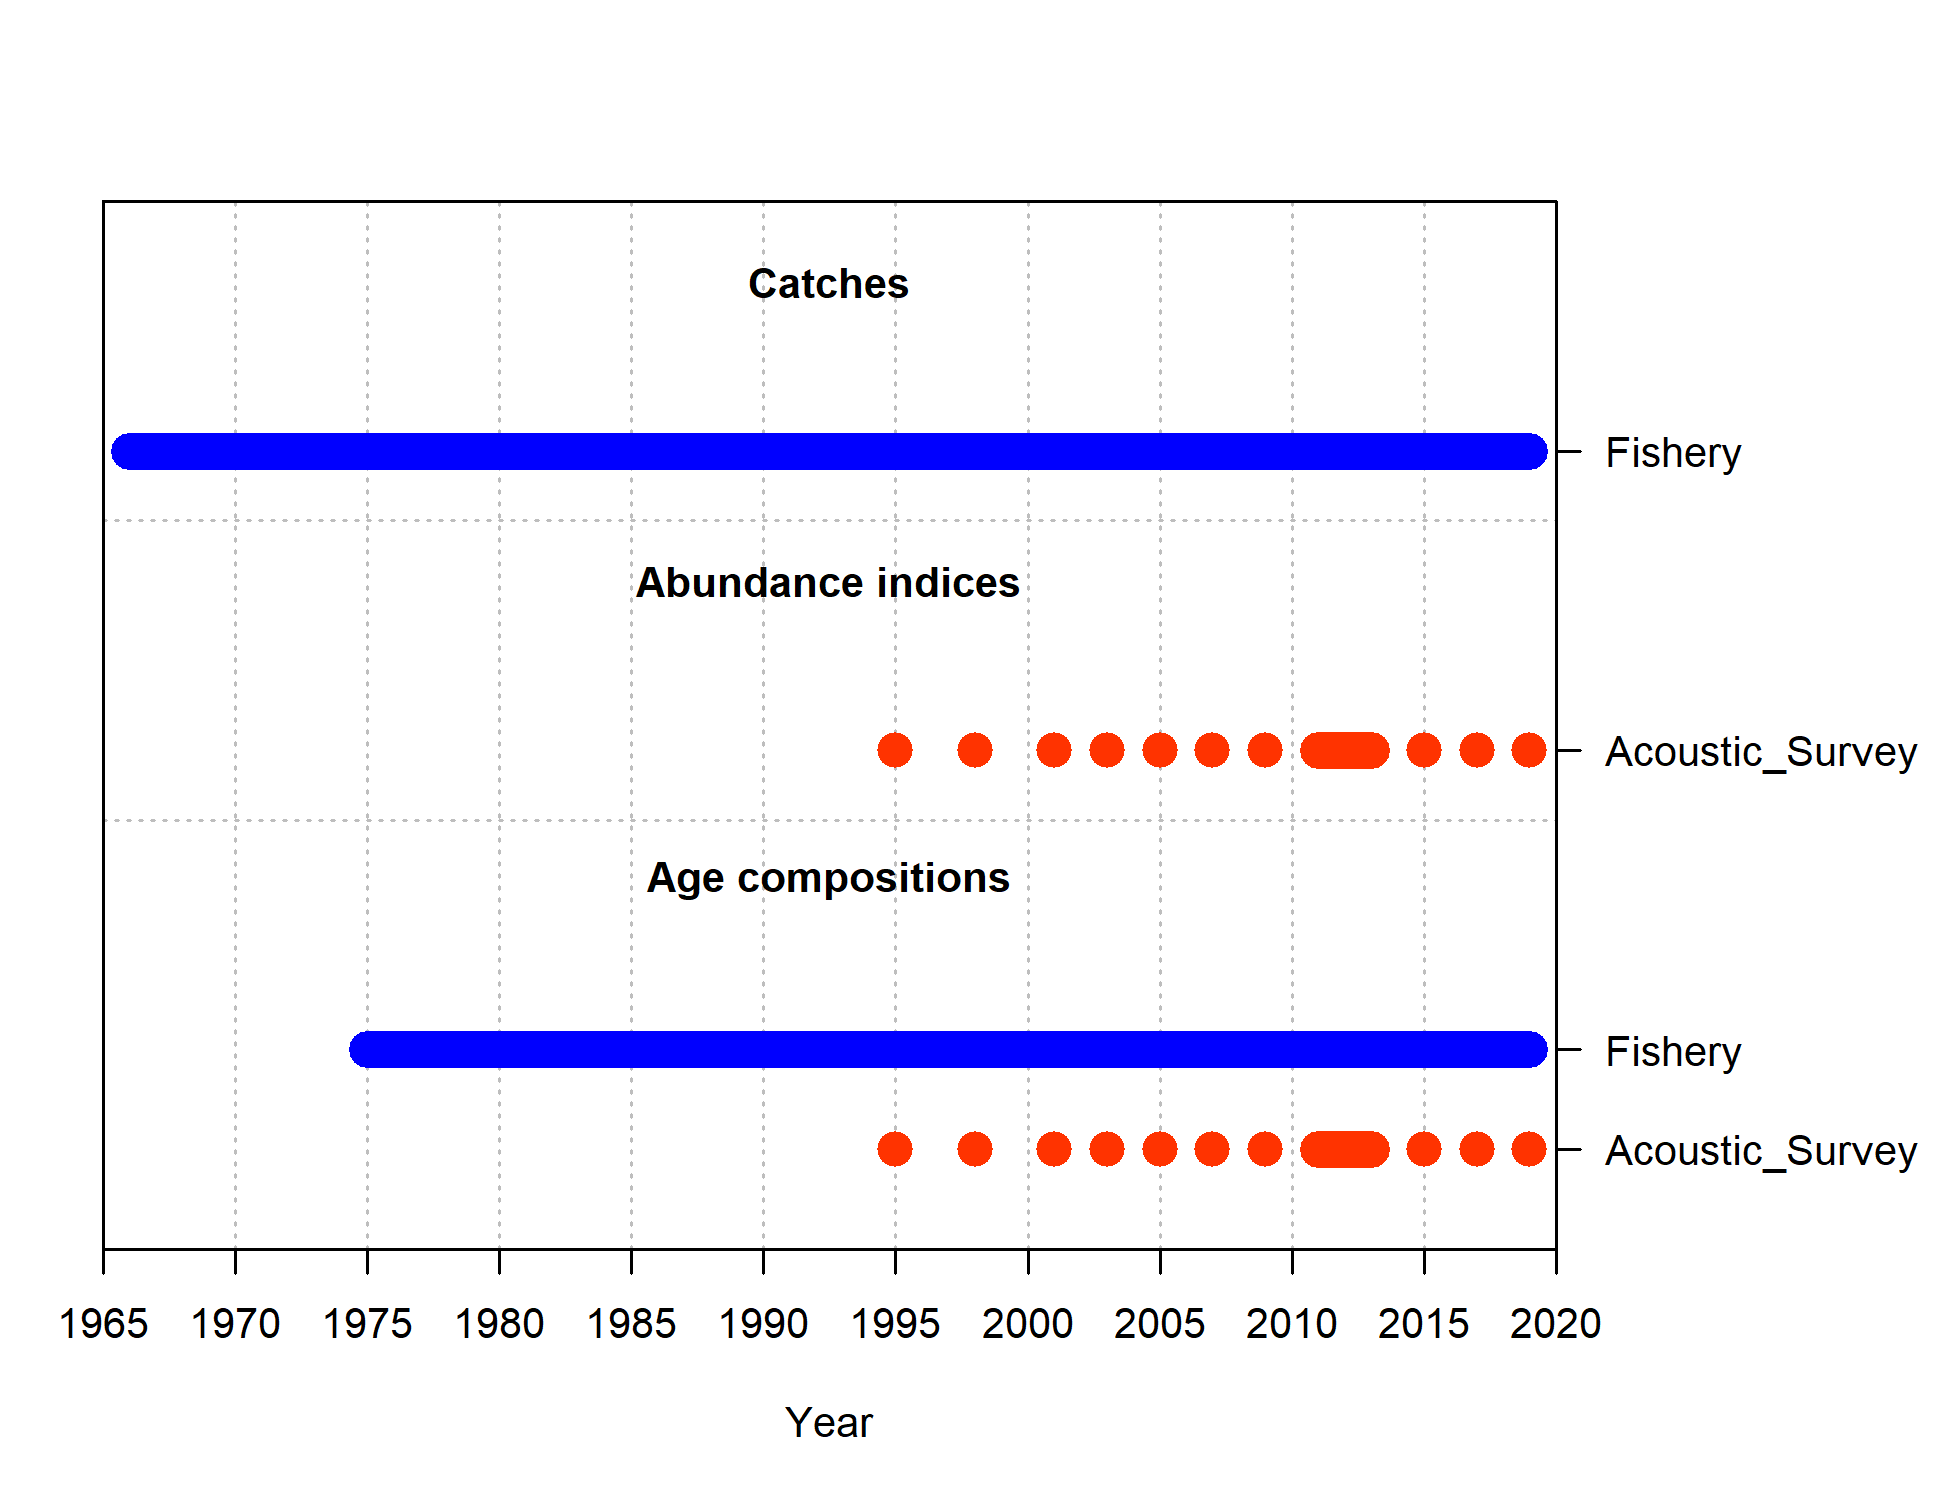
\includegraphics[width=1\textwidth,height=1\textheight]{data-plot.png}
\caption{Summary of data sources used in the base model.\label{fig:data-plot}}
\end{figure}

\tagmcend\tagstructend

\tagstructbegin{tag=H1}\tagmcbegin{tag=H1}

\hypertarget{appendix-model-description}{%
\section{Appendix model description}\label{appendix-model-description}}

\leavevmode\tagmcend\tagstructend

\tagstructbegin{tag=H2}\tagmcbegin{tag=H2}

\hypertarget{dynamics}{%
\subsection{Dynamics}\label{dynamics}}

\leavevmode\tagmcend\tagstructend

\tagstructbegin{tag=P}\tagmcbegin{tag=P}

This assessment is based on a statistical age-structured model with the catch equation and population dynamics model as described in Fournier and Archibald (1982) and elsewhere (e.g., Hilborn and Walters 1992, Schnute and Richards 1995, McAllister and Ianelli 1997). The catch in numbers at age in year {\tagstructbegin{tag=Formula}\tagmcbegin{tag=Formula}\(t (C_{t,a})\)\leavevmode\tagmcend\tagstructend} and total catch biomass {\tagstructbegin{tag=Formula}\tagmcbegin{tag=Formula}\((Y_t)\)\leavevmode\tagmcend\tagstructend} can be described as:

\leavevmode\tagmcend\tagstructend\par

\tagstructbegin{tag=P}\tagmcbegin{tag=P}

\begin{align}
    C_{t,a}     &= \frac{F_{t,a}}{Z_{t,a}} \left(1 - e^{-Z_{t,a}}\right) N_{t,a}, &1 \le t \le T, 1 \le a \le A \\
    N_{t+1,a+1} &= N_{t,a-1} e^{-Z_{t,a-1}}                                       &1 \le t \le T, 1 \le a < A   \\
    N_{t+1,A}   &= N_{t,A-1} e^{-Z_{t,A-1}} + N_{t,A} e^{-Z_{t,A}} ,              &1 \le t \le T                \\
    Z_{t,a}     &= F_{t,a} + M_{t,a}                                                                            \\
    C_{t,.}     &= \sum_{a=1}^A{C_{t,a}}                                                                        \\
    p_{t,a}     &= \frac{C_{t,a} } {C_{t,.} }                                                                   \\
    Y_{t}       &= \sum_{a=1}^A{w_{t,a}C_{t,a}}                                                                 \\
\end{align}

\leavevmode\tagmcend\tagstructend\par

where

\tagstructbegin{tag=P}\tagmcbegin{tag=P}

Fishing mortality ({\tagstructbegin{tag=Formula}\tagmcbegin{tag=Formula}\(F_{t,a}\)\leavevmode\tagmcend\tagstructend}) is specified as being semi-separable and non-parametric in form with restrictions on the variability following Butterworth et al.~(2003):

\leavevmode\tagmcend\tagstructend\par

\tagstructbegin{tag=P}\tagmcbegin{tag=P}

\begin{align}
    F_{t,a}     &= s_{t,a} \, \mu^f e^{\epsilon_t}, &\epsilon_t   \sim \mathcal{N}(0,\,\sigma_E^{2}) \\
    s_{t+1,a}   &= s_{t,a} \,       e^{\gamma_t},   &\gamma_t     \sim \mathcal{N}(0,\,\sigma_s^{2}) 
\end{align}

\leavevmode\tagmcend\tagstructend\par

\tagstructbegin{tag=P}\tagmcbegin{tag=P}

where {\tagstructbegin{tag=Formula}\tagmcbegin{tag=Formula}\(s_{t,a}\)\leavevmode\tagmcend\tagstructend} is the selectivity for age class {\tagstructbegin{tag=Formula}\tagmcbegin{tag=Formula}\(a\)\leavevmode\tagmcend\tagstructend} in year {\tagstructbegin{tag=Formula}\tagmcbegin{tag=Formula}\(t\)\leavevmode\tagmcend\tagstructend}, and {\tagstructbegin{tag=Formula}\tagmcbegin{tag=Formula}\(\mu^f\)\leavevmode\tagmcend\tagstructend} is the median fishing mortality rate over time.

\leavevmode\tagmcend\tagstructend\par

\tagstructbegin{tag=P}\tagmcbegin{tag=P}

If the selectivities ({\tagstructbegin{tag=Formula}\tagmcbegin{tag=Formula}\(s_{t,a}\)\leavevmode\tagmcend\tagstructend}) are constant over time then fishing mortality rate decomposes into an age component and a year component. A curvature penalty on the selectivity coefficients using the squared second-differences to provide smoothness between ages.

\leavevmode\tagmcend\tagstructend\par

\tagstructbegin{tag=P}\tagmcbegin{tag=P}

Bottom-trawl survey selectivity was set to be asymptotic yet retain the properties desired for the characteristics of this gear. Namely, that the function should allow flexibility in selecting age 1 pollock over time. The functional form of this selectivity was:

\leavevmode\tagmcend\tagstructend\par

\tagstructbegin{tag=P}\tagmcbegin{tag=P}

\begin{align}
    s_{t,a}     &= \left[ 1+e^{-\alpha_ta-\beta_t} \right]^{-1} , & a>1 \\
    s_{t,a}     &= \mu_se^{-\delta^\mu_t},                        & a=1 \\
    \alpha_{t}  &= \bar \alpha e^{\delta^\alpha_t},                     \\
    \beta_{t}  &= \bar \beta e^{\delta^\beta_t},                        
\end{align}

\leavevmode\tagmcend\tagstructend\par

\tagstructbegin{tag=P}\tagmcbegin{tag=P}

where the parameters of the selectivity function follow a random walk process as in Dorn et al.~(2000):

\leavevmode\tagmcend\tagstructend\par

\tagstructbegin{tag=P}\tagmcbegin{tag=P}

\begin{align}
    \delta_t^\mu  -  \delta_{t+1}^\mu     &\sim \mathcal{N}(0,\,\sigma_{\delta^\mu}^{2}) \\
    \\
    \alpha_t^\mu  -  \alpha_{t+1}^\mu     &\sim \mathcal{N}(0,\,\sigma_{\alpha^\mu}^{2}) \\
    \beta_t^\mu  -  \beta_{t+1}^\mu     &\sim \mathcal{N}(0,\,\sigma_{\beta^\mu}^{2}) 
\end{align}

\leavevmode\tagmcend\tagstructend\par

\tagstructbegin{tag=P}\tagmcbegin{tag=P}

The variance terms for these process error parameters were specified to be 0.04.

\leavevmode\tagmcend\tagstructend\par

\tagstructbegin{tag=P}\tagmcbegin{tag=P}

In this assessment, the random-walk deviation penalty was optionally shifted to the changes in log-selectivity. that is, for the BTS estimates, the process error was applied to the logistic parameters as above, but the lognormal penalty was applied to the resulting selectivities-at-age directly. The extent of this variability was evaluated in the context of the impact on age-specific survey catchability/availability and contrasted with an independent estimate of pollock availability to the bottom trawl survey. \begin{align}
    {ln(s_{t,a})}  -  {ln(s_{t+1,a})}  &\sim \mathcal{N}(0,\,\sigma_{sel}^{2}) \\
\end{align} In 2008 the AT survey selectivity approach was modified. As an option, the age one pollock observed in this trawl can be treated as an index and are not considered part of the age composition (which then ranges from age 2-15). This was done to improve some interaction with the flexible selectivity smoother that is used for this gear and was compared. Additionally, the annual specification of input observation variance terms was allowed for the AT data.

\leavevmode\tagmcend\tagstructend\par

\tagstructbegin{tag=P}\tagmcbegin{tag=P}

A diagnostic approach to evaluate input variance specifications (via sample size under multinomial assumptions) was added in the 2018 assessment. This method uses residuals from mean ages together with the concept that the sample variance of mean age (from a given annual data set) varies inversely with input sample size. It can be shown that for a given set of input proportions at age (up to the maximum age {\tagstructbegin{tag=Formula}\tagmcbegin{tag=Formula}\(A\)\leavevmode\tagmcend\tagstructend}) and sample size {\tagstructbegin{tag=Formula}\tagmcbegin{tag=Formula}\(N_t\)\leavevmode\tagmcend\tagstructend} for year {\tagstructbegin{tag=Formula}\tagmcbegin{tag=Formula}\(t\)\leavevmode\tagmcend\tagstructend}, an adjustment factor {\tagstructbegin{tag=Formula}\tagmcbegin{tag=Formula}\(\nu\)\leavevmode\tagmcend\tagstructend} for input sample size can be computed when compared with the assessment model predicted proportions at age ({\tagstructbegin{tag=Formula}\tagmcbegin{tag=Formula}\(\hat p_{ta}\)\leavevmode\tagmcend\tagstructend}) and model predicted mean age ({\tagstructbegin{tag=Formula}\tagmcbegin{tag=Formula}\(\hat{\bar{a_t}}\)\leavevmode\tagmcend\tagstructend}): \begin{align}
\nu   &= \text{var}\left( r^a_t \sqrt{\frac{N_t}{\kappa_t} }\right)^{-1} \\
r^a_t &= \bar a_t - \hat{\bar{a_t}}                                      \\
\kappa_t &= \left[ \sum_a^A {\bar a_t - \hat{\bar{a_t}}} \right]^{0.5}
\end{align}

\leavevmode\tagmcend\tagstructend\par

\tagstructbegin{tag=P}\tagmcbegin{tag=P}

where {\tagstructbegin{tag=Formula}\tagmcbegin{tag=Formula}\(r^a_t\)\leavevmode\tagmcend\tagstructend} is the residual of mean age and \begin{align}
\hat{\bar{a_t}} &= \sum_a^A{a \hat p_{ta}}\, \\
{\bar a_t}      &= \sum_a^A{a p_{ta}}\, 
\end{align}

\leavevmode\tagmcend\tagstructend\par

\tagstructbegin{tag=P}\tagmcbegin{tag=P}

Based on previous analyses, we used the above relationship as a diagnostic for evaluating input sample sizes by comparing model predicted mean ages with observed mean ages and the implied 95\% confidence bands. This method provided support for modifying the frequency of allowing selectivity changes.

\leavevmode\tagmcend\tagstructend\par

\tagstructbegin{tag=H2}\tagmcbegin{tag=H2}

\hypertarget{recruitment-1}{%
\subsection{Recruitment}\label{recruitment-1}}

\leavevmode\tagmcend\tagstructend

\tagstructbegin{tag=P}\tagmcbegin{tag=P}

In these analyses, recruitment ({\tagstructbegin{tag=Formula}\tagmcbegin{tag=Formula}\(R_t\)\leavevmode\tagmcend\tagstructend}) represents numbers of age-1 individuals modeled as a stochastic function of spawning stock biomass. \begin{align}
        R_t = f\left(B_{t-1} \right)
\end{align} with mature spawning biomass during year {\tagstructbegin{tag=Formula}\tagmcbegin{tag=Formula}\(t\)\leavevmode\tagmcend\tagstructend} was defined as: \begin{align}
  B_t = \sum_{a=1}^A{ w_{t,a}\phi_aN_{t,a}} 
\end{align}

\leavevmode\tagmcend\tagstructend\par

\tagstructbegin{tag=P}\tagmcbegin{tag=P}

and, {\tagstructbegin{tag=Formula}\tagmcbegin{tag=Formula}\(\phi_a\)\leavevmode\tagmcend\tagstructend} is the proportion of mature females at age is as shown in the sub-section titled Natural mortality and maturity at age under ``Parameters estimated independently'' above.

\leavevmode\tagmcend\tagstructend\par

\tagstructbegin{tag=P}\tagmcbegin{tag=P}

A reparameterized form for the stock-recruitment relationship following Francis (1992) was used. For the optional Beverton-Holt form (the Ricker form presented in Eq. 12 was adopted for this assessment) we have: \begin{align}
R_t &= \frac{B_{t-1}e^{\varepsilon_t} }{\alpha+\beta B_{t-1} }
\end{align}

\leavevmode\tagmcend\tagstructend\par

where

\tagstructbegin{tag=P}\tagmcbegin{tag=P}

Values for the stock-recruitment function parameters and are calculated from the values of (the number of 0-year-olds in the absence of exploitation and recruitment variability) and the steepness of the stock-recruit relationship ({\tagstructbegin{tag=Formula}\tagmcbegin{tag=Formula}\(h\)\leavevmode\tagmcend\tagstructend}). The steepness is the fraction of R0 to be expected (in the absence of recruitment variability) when the mature biomass is reduced to 20\% of its pristine level (Francis 1992), so that:

\leavevmode\tagmcend\tagstructend\par

\tagstructbegin{tag=P}\tagmcbegin{tag=P}

\begin{align}
 \alpha &= \tilde B_0 \frac{1-h}{4h} \\
 \beta &= \frac{5h-1}{4hR_0 } 
\end{align}

\leavevmode\tagmcend\tagstructend\par

\tagstructbegin{tag=P}\tagmcbegin{tag=P}

where {\tagstructbegin{tag=Formula}\tagmcbegin{tag=Formula}\(\tilde B_0\)\leavevmode\tagmcend\tagstructend} is the total egg production (or proxy, e.g., female spawning biomass) in the absence of exploitation (and recruitment variability) expressed as a fraction of {\tagstructbegin{tag=Formula}\tagmcbegin{tag=Formula}\(R_0\)\leavevmode\tagmcend\tagstructend}.

\leavevmode\tagmcend\tagstructend\par

\tagstructbegin{tag=P}\tagmcbegin{tag=P}

Some interpretation and further explanation follows. For steepness equal 0.2, then recruits are a linear function of spawning biomass (implying no surplus production). For steepness equal to 1.0, then recruitment is constant for all levels of spawning stock size. A value of {\tagstructbegin{tag=Formula}\tagmcbegin{tag=Formula}\(h = 0.9\)\leavevmode\tagmcend\tagstructend} implies that at 20\% of the unfished spawning stock size will result in an expected value of 90\% unfished recruitment level. Steepness of 0.7 is a commonly assumed default value for the Beverton-Holt form (e.g., Kimura 1988). The prior distribution for steepness used a beta distribution as in Ianelli et al.~(2016). The prior on steepness was specified to be a symmetric form of the Beta distribution with {\tagstructbegin{tag=Formula}\tagmcbegin{tag=Formula}\(\alpha = \beta = 14.93\)\leavevmode\tagmcend\tagstructend} implying a prior mean of 0.5 and CV of 12\% (implying that there is about a 14\% chance that the steepness is greater than 0.6). This conservative prior is consistent with previous years' application and serves to constrain the stock-recruitment curve from favoring steep slopes (uninformative priors result in {\tagstructbegin{tag=Formula}\tagmcbegin{tag=Formula}\(F_{MSY}\)\leavevmode\tagmcend\tagstructend} values near an {\tagstructbegin{tag=Formula}\tagmcbegin{tag=Formula}\(F_{SPR}\)\leavevmode\tagmcend\tagstructend} of about {\tagstructbegin{tag=Formula}\tagmcbegin{tag=Formula}\(F_{18\%}\)\leavevmode\tagmcend\tagstructend} a value considerably higher than the default proxy of {\tagstructbegin{tag=Formula}\tagmcbegin{tag=Formula}\(F_{35\%}\)\leavevmode\tagmcend\tagstructend}). The residual pattern for the post-1977 recruits used in fitting the curve with a more diffuse prior resulted in all estimated recruits being below the curve for stock sizes less than {\tagstructbegin{tag=Formula}\tagmcbegin{tag=Formula}\(B_{MSY}\)\leavevmode\tagmcend\tagstructend} (except for the 1978 year class). We believe this to be driven primarily by the apparent negative-slope for recruits relative to stock sizes above {\tagstructbegin{tag=Formula}\tagmcbegin{tag=Formula}\(B_{MSY}\)\leavevmode\tagmcend\tagstructend} and as such, provides a potentially unrealistic estimate of productivity at low stock sizes. This prior was elicited from the rationale that residuals should be reasonably balanced throughout the range of spawning stock sizes. Whereas this is somewhat circular (i.e., using data for prior elicitation), the point here is that residual patterns (typically ignored in these types of models) were qualitatively considered.

\leavevmode\tagmcend\tagstructend\par

\tagstructbegin{tag=P}\tagmcbegin{tag=P}

In model 16.1 (from the 2019 assessment), a Beverton Holt stock recruitment form was implemented using the prior value of 0.67 for steepness and a CV of 0.17. This resulted in beta distribution parameters (for the prior) at {\tagstructbegin{tag=Formula}\tagmcbegin{tag=Formula}\(\alpha = 6.339\)\leavevmode\tagmcend\tagstructend} and\\
{\tagstructbegin{tag=Formula}\tagmcbegin{tag=Formula}\(\beta = 4.293\)\leavevmode\tagmcend\tagstructend}.

\leavevmode\tagmcend\tagstructend\par

\tagstructbegin{tag=P}\tagmcbegin{tag=P}

The value of {\tagstructbegin{tag=Formula}\tagmcbegin{tag=Formula}\(\sigma_R\)\leavevmode\tagmcend\tagstructend} was set at 1.0 to accommodate additional uncertainty in factors affecting recruitment variability.

\leavevmode\tagmcend\tagstructend\par

\tagstructbegin{tag=P}\tagmcbegin{tag=P}

To have the critical value for the stock-recruitment function (steepness, \emph{h}) on the same scale for the Ricker model, we begin with the parameterization of Kimura (1990): \begin{align}
R_t &= \frac{B_{t-1}e^{\alpha \left(1-B_{t-1} \frac{R_0}{\psi_0} \right)}}{\psi_0}
\end{align}

\leavevmode\tagmcend\tagstructend\par

\tagstructbegin{tag=P}\tagmcbegin{tag=P}

It can be shown that the Ricker parameter a maps to steepness as: \begin{align}
h &= \frac{e^\alpha}{e^\alpha+4}
\end{align}

\leavevmode\tagmcend\tagstructend\par

\tagstructbegin{tag=P}\tagmcbegin{tag=P}

so that the prior used on \emph{h} can be implemented in both the Ricker and Beverton-Holt stock-recruitment forms. Here the term {\tagstructbegin{tag=Formula}\tagmcbegin{tag=Formula}\(\psi_0\)\leavevmode\tagmcend\tagstructend} represents the equilibrium unfished spawning biomass per-recruit.

\leavevmode\tagmcend\tagstructend\par

\tagstructbegin{tag=H2}\tagmcbegin{tag=H2}

\hypertarget{diagnostics}{%
\subsection{Diagnostics}\label{diagnostics}}

\leavevmode\tagmcend\tagstructend

\tagstructbegin{tag=P}\tagmcbegin{tag=P}

In 2006 a replay feature was added where the time series of recruitment estimates from a particular model is used to compute the subsequent abundance expectation had no fishing occurred. These recruitments are adjusted from the original estimates by the ratio of the expected recruitment given spawning biomass (with and without fishing) and the estimated stock-recruitment curve. I.e., the recruitment under no fishing is modified as: {\tagstructbegin{tag=Formula}\tagmcbegin{tag=Formula}\[R_t' = \hat{R}_t\frac{f(B_{t-1}')}{f(B_{t-1})}\]\leavevmode\tagmcend\tagstructend} where {\tagstructbegin{tag=Formula}\tagmcbegin{tag=Formula}\(R_t\)\leavevmode\tagmcend\tagstructend} is the original recruitment estimate in year {\tagstructbegin{tag=Formula}\tagmcbegin{tag=Formula}\(t\)\leavevmode\tagmcend\tagstructend} with {\tagstructbegin{tag=Formula}\tagmcbegin{tag=Formula}\(B_{t-1}'\)\leavevmode\tagmcend\tagstructend} and {\tagstructbegin{tag=Formula}\tagmcbegin{tag=Formula}\(B_{t-1}\)\leavevmode\tagmcend\tagstructend} representing the stock-recruitment function given spawning biomass under no fishing and under the estimated fishing intensity, respectively.

\leavevmode\tagmcend\tagstructend\par

\tagstructbegin{tag=P}\tagmcbegin{tag=P}

The assessment model code allows retrospective analyses (e.g., Parma 1993, and Ianelli and Fournier 1998). This was designed to assist in specifying how spawning biomass patterns (and uncertainty) have changed due to new data. The retrospective approach simply uses the current model to evaluate how it may change over time with the addition of new data based on the evolution of data collected over the past several years.

\leavevmode\tagmcend\tagstructend\par

\tagstructbegin{tag=H2}\tagmcbegin{tag=H2}

\hypertarget{parameter-estimation}{%
\subsection{Parameter estimation}\label{parameter-estimation}}

\leavevmode\tagmcend\tagstructend

\tagstructbegin{tag=P}\tagmcbegin{tag=P}

The objective function was simply the sum of the negative log-likelihood function and logs of the prior distributions. To fit large numbers of parameters in nonlinear models it is useful to be able to estimate certain parameters in different stages. The ability to estimate stages is also important in using robust likelihood functions since it is often undesirable to use robust objective functions when models are far from a solution. Consequently, in the early stages of estimation we use the following log- likelihood function for the survey and fishery catch at age data (in numbers):

\leavevmode\tagmcend\tagstructend\par

\tagstructbegin{tag=P}\tagmcbegin{tag=P}

\begin{align}
nll(i) &= n \sum_{t,a}{ p_{ta} \ln \hat p_{ta} } \\
p_{ta} &= \frac{O_{ta}}{\sum_a{O_{ta}}} \hspace{20pt} 
\hat p_{ta} = \frac{\hat C_{ta}}{\sum_a{\hat C_{ta}}} \\
\mathbf{C} &= \mathbf{CE}  \\
\mathbf{E}  &=  \begin{array}{llll} 
b_{1,1} & b_{1,2} & \dots & b_{1,15} \\
b_{2,1} & b_{2,2} &       & b_{2,15} \\
\vdots &         & \ddots &  \vdots \\
b_{15,1} & b_{15,2} & \dots      & b_{15,15} 
\end{array}  
\end{align}

\leavevmode\tagmcend\tagstructend\par

\tagstructbegin{tag=P}\tagmcbegin{tag=P}

where {\tagstructbegin{tag=Formula}\tagmcbegin{tag=Formula}\(A\)\leavevmode\tagmcend\tagstructend}, and {\tagstructbegin{tag=Formula}\tagmcbegin{tag=Formula}\(T\)\leavevmode\tagmcend\tagstructend}, represent the number of age classes and years, respectively, n is the sample size, and represent the observed and predicted numbers at age in the catch. The elements bi,j represent ageing mis-classification proportions are based on independent agreement rates between otolith age readers. For the models presented this year, the option for including aging errors was re-evaluated.

\leavevmode\tagmcend\tagstructend\par

\tagstructbegin{tag=P}\tagmcbegin{tag=P}

Sample size values were revised and are shown in the main document. Strictly speaking, the amount of data collected for this fishery indicates higher values might be warranted. However, the standard multinomial sampling process is not robust to violations of assumptions (Fournier et al.~1990). Consequently, as the model fit approached a solution, we invoke a robust likelihood function which fit proportions at age as:

\leavevmode\tagmcend\tagstructend\par

\tagstructbegin{tag=P}\tagmcbegin{tag=P}

\begin{align}
\prod_{a=1}^A\prod_{t=1}^T \left[\left( \exp{\left(-\frac{\left(p_{ta}-\hat p_{ta}\right)^2}{2\left(\eta_{ta}+0.1/A\right)\tau_t^2} \right)
}+0.01 \right) \times  \frac{1}{ {\sqrt{2\pi \left ( \eta_{ta}+0.1/A \right) \tau_t}} } \right]
\end{align}

\leavevmode\tagmcend\tagstructend\par

\tagstructbegin{tag=P}\tagmcbegin{tag=P}

Taking the logarithm we obtain the log-likelihood function for the age composition data:

\leavevmode\tagmcend\tagstructend\par

\tagstructbegin{tag=P}\tagmcbegin{tag=P}

\begin{align}
nll(i) = -0.5\sum_{a=1}^A\sum_{t=1}^T{
{\ln{2\pi \left( \eta_{ta}+0.1/A \right) 
-\sum_t^T A\ln\tau_t}} } 
+\sum_{a=1}^A\sum_{t=1}^T{\ln\left\{
\exp{\left(-\frac{\left(p_{ta}-\hat p_{ta}\right)^2}{\left(2\eta_{ta}+0.1/A\right)\tau_t^2} \right)
+ 0.01 } 
\right\}}
\end{align}

\leavevmode\tagmcend\tagstructend\par

\tagstructbegin{tag=P}\tagmcbegin{tag=P}

where \begin{align}
\eta_{ta} &=  p_{ta}(1-p_{ta})\\ 
\text{and} \\
\tau_t^2 &=  1/n_t 
\end{align} which gives the variance for {\tagstructbegin{tag=Formula}\tagmcbegin{tag=Formula}\(p_{ta}\)\leavevmode\tagmcend\tagstructend} \begin{align}
(\eta_{ta}+0.1/A)\tau_t^2
\end{align}

\leavevmode\tagmcend\tagstructend\par

\tagstructbegin{tag=P}\tagmcbegin{tag=P}

Completing the estimation in this fashion reduces the model sensitivity to data that would otherwise be considered outliers.

\leavevmode\tagmcend\tagstructend\par

\tagstructbegin{tag=P}\tagmcbegin{tag=P}

Within the model, predicted survey abundance accounted for within-year mortality since surveys occur during the middle of the year. As in previous years, we assumed that removals by the survey were insignificant (i.e., the mortality of pollock caused by the survey was considered insignificant). Consequently, a set of analogous catchability and selectivity terms were estimated for fitting the survey observations as:

\leavevmode\tagmcend\tagstructend\par

\tagstructbegin{tag=P}\tagmcbegin{tag=P}

\begin{align}
\hat N_{ta}^s &= e^{-0.5Z_{ta}}N_{ta}q_t^ss_{ta}^S
\end{align}

\leavevmode\tagmcend\tagstructend\par

\tagstructbegin{tag=P}\tagmcbegin{tag=P}

where the superscript s indexes the type of survey (AT or BTS). For the option to use the survey predictions in biomass terms instead of just abundance, the above was modified to include observed survey biomass weights-at-age:

\leavevmode\tagmcend\tagstructend\par

\tagstructbegin{tag=P}\tagmcbegin{tag=P}

\begin{align}
\hat N_{ta}^s &= e^{-0.5Z_{ta}}w_{ta}N_{ta}q_t^ss_{ta}^S
\end{align}

\leavevmode\tagmcend\tagstructend\par

\tagstructbegin{tag=P}\tagmcbegin{tag=P}

For the AVO index, the values for selectivity were assumed to be the same as for the AT survey and the mean weights at age over time was also assumed to be equal to the values estimated for the AT survey.

\leavevmode\tagmcend\tagstructend\par

\tagstructbegin{tag=P}\tagmcbegin{tag=P}

For these analyses we chose to keep survey catchabilities constant over time (though they are estimated separately for the AVO index and for the AT and bottom trawl surveys). The contribution to the negative log-likelihood function (ignoring constants) from the surveys is given by either the lognormal distribution:

\leavevmode\tagmcend\tagstructend\par

\tagstructbegin{tag=P}\tagmcbegin{tag=P}

\begin{align}
nll(i) &= \sum_t{\frac{\ln(u_t^s/\hat N_t^s)^2}{2\sigma_{s,t}^2}}
\end{align} where {\tagstructbegin{tag=Formula}\tagmcbegin{tag=Formula}\(u_t^s\)\leavevmode\tagmcend\tagstructend} is the total (numerical abundance or optionally biomass) estimate with variance {\tagstructbegin{tag=Formula}\tagmcbegin{tag=Formula}\(\sigma_{s,t}\)\leavevmode\tagmcend\tagstructend} from survey {\tagstructbegin{tag=Formula}\tagmcbegin{tag=Formula}\(s\)\leavevmode\tagmcend\tagstructend} in year {\tagstructbegin{tag=Formula}\tagmcbegin{tag=Formula}\(t\)\leavevmode\tagmcend\tagstructend} or optionally, the normal distribution can be selected: \begin{align}
nll(i) &= \sum_t{\frac{(u_t^s - \hat N_t^s)^2}{2\sigma_{s,t}^2}}. \\
\end{align}

\leavevmode\tagmcend\tagstructend\par

\tagstructbegin{tag=P}\tagmcbegin{tag=P}

The AT survey and AVO index is modeled using a lognormal distribution whereas for the BTS survey, a normal distribution was applied.

\leavevmode\tagmcend\tagstructend\par

\tagstructbegin{tag=P}\tagmcbegin{tag=P}

For model configurations in which the BTS data are corrected for estimated efficiency, a multivariate lognormal distribution was used. For the negative- log likelihood component this was modeled as \begin{equation}
nll_i = 0.5\mathbf{X}\Sigma^{-1}\mathbf{X}^{'}
\end{equation}

\leavevmode\tagmcend\tagstructend\par

\tagstructbegin{tag=P}\tagmcbegin{tag=P}

where is a vector of observed minus model predicted values for this index and {\tagstructbegin{tag=Formula}\tagmcbegin{tag=Formula}\(\Sigma\)\leavevmode\tagmcend\tagstructend} is the estimated covariance matrix provided from the method provided in Kotwicki et al.~2014. For the VAST estimates, the supplied covariance matrix was used in the same way.

\leavevmode\tagmcend\tagstructend\par

\tagstructbegin{tag=P}\tagmcbegin{tag=P}

The contribution to the negative log-likelihood function for the observed total catch biomass ({\tagstructbegin{tag=Formula}\tagmcbegin{tag=Formula}\(C_b^{obs}, \hat{C_b}\)\leavevmode\tagmcend\tagstructend}) by the fishery is given by \begin{equation}
nll_i = 0.5\sum_t\frac{\ln(C_b^{obs}/\hat C_b)^2}{2\sigma_{C_b,t}^2}
\end{equation}

\leavevmode\tagmcend\tagstructend\par

\tagstructbegin{tag=P}\tagmcbegin{tag=P}

where {\tagstructbegin{tag=Formula}\tagmcbegin{tag=Formula}\(\sigma_{C_b,t}\)\leavevmode\tagmcend\tagstructend} is pre-specified (set to 0.05) reflecting the accuracy of the overall observed catch in biomass. Similarly, the contribution of prior distributions (in negative log-density) to the log-likelihood function include {\tagstructbegin{tag=Formula}\tagmcbegin{tag=Formula}\(\lambda_\varepsilon \sum_t\varepsilon_t^2 +\lambda_\gamma \sum_{ta}\gamma^2 + \lambda_\delta \sum_t\delta_t^2\)\leavevmode\tagmcend\tagstructend} where the size of the 's represent prior assumptions about the variances of these random variables. Most of these parameters are associated with year-to- year and age specific deviations in selectivity coefficients. For a presentation of this type of Bayesian approach to modeling errors-in- variables, the reader is referred to Schnute (1994). To facilitate estimating such a large number of parameters, automatic differentiation software extended from Greiwank and Corliss (1991) and developed into C++ class libraries was used. This software provided the derivative calculations needed for finding the posterior mode via a quasi-Newton function minimization routine (e.g., Press et al.~1992). The model implementation language (ADModel Builder) gave simple and rapid access to these routines and provided the ability estimate the variance-covariance matrix for all dependent and independent parameters of interest.

\leavevmode\tagmcend\tagstructend\par
\end{document}
